\documentclass[10.5pt,a4paper]{article}
\usepackage[top=1.6cm,bottom=1.6cm,left=1.8cm,right=1.8cm]{geometry}
\usepackage[utf8]{inputenc}
\usepackage[T1]{fontenc}
\usepackage[french]{babel}
\usepackage{lmodern}
\usepackage{xcolor}
\usepackage{graphicx}
\usepackage{titlesec}
\usepackage{enumitem}
\usepackage{array}
\usepackage{tabularx}
\usepackage{booktabs}
\usepackage{hyperref}
\usepackage{fancyhdr}
\usepackage{lastpage}

\definecolor{agirhindigo}{HTML}{4F46E5}
\definecolor{agirhdark}{HTML}{1E1B4B}
\definecolor{agirhbg}{HTML}{EEF2FF}

\hypersetup{colorlinks=true,linkcolor=agirhindigo,urlcolor=agirhindigo,citecolor=agirhindigo}

\setlength{\parindent}{0pt}
\setlength{\parskip}{4.5pt}

\titleformat{\section}{\large\bfseries\color{agirhindigo}}{\thesection.}{0.5em}{}
\titlespacing*{\section}{0pt}{7pt}{3pt}
\titleformat{\subsection}{\normalsize\bfseries\color{agirhdark}}{\thesubsection}{0.5em}{}
\titlespacing*{\subsection}{0pt}{5pt}{2pt}

\setlist[itemize]{topsep=1pt,itemsep=1pt,parsep=0pt,leftmargin=1.3em}
\setlist[enumerate]{topsep=1pt,itemsep=1pt,parsep=0pt,leftmargin=1.5em}

\pagestyle{fancy}
\fancyhf{}
\renewcommand{\headrulewidth}{0.4pt}
\fancyhead[L]{\footnotesize\color{gray} AGIRH --- Rapport d'\'Etat d'Avancement}
\fancyhead[R]{\footnotesize\color{gray} Wilfried TSETSE --- ENSA Safi}
\fancyfoot[C]{\footnotesize\color{gray} \thepage/\pageref{LastPage}}

\newcommand{\code}[1]{\texttt{\small #1}}

\begin{document}

% ---------- Bandeau titre compact ----------
\begin{center}
  {\Large\bfseries\color{agirhindigo} AGIRH --- Rapport d'\'Etat d'Avancement}\\[2pt]
  {\normalsize Agent RH agentique pour l'Onboarding et l'Offboarding --- ENSA Safi, GIDIA}\\[4pt]
  {\small
    \begin{tabularx}{\textwidth}{@{}X X@{}}
      \textbf{R\'ealis\'e par} : M. Komla Edem Wilfried Tsetse &
      \textbf{Encadrant} : M. Moulay Rachid Didi Alaoui (superviseur) \\
    \end{tabularx}
  }\\[2pt]
  {\footnotesize Ann\'ee universitaire 2025--2026}
\end{center}
\vspace{2pt}
\hrule
\vspace{4pt}

% ---------- 1. Contexte ----------
\section{Contexte et strat\'egie}

Le stage vise la r\'ealisation d'un agent conversationnel d\'edi\'e \`a l'onboarding et \`a l'offboarding des collaborateurs : r\'epondre aux questions sur les politiques internes (RAG document\'e) et informer sur l'avancement d'un dossier, \textbf{sans jamais ex\'ecuter d'action destructrice ou irr\'eversible} depuis la conversation --- une contrainte de conception assum\'ee, pas une limite technique.

Une premi\`ere it\'eration architecturale a \'et\'e r\'e-audit\'ee en cours de stage : pipeline RAG sans reranking ni index vectoriel d\'edi\'e, boucle d'auto-correction non fonctionnelle en configuration r\'eelle (bug de bouclage confirm\'e en code), et un p\'erim\`etre m\'etier qui d\'erivait au-del\`a du sujet r\'eel. Une refonte cibl\'ee a \'et\'e men\'ee pour corriger ces limites et recentrer strictement le p\'erim\`etre sur l'onboarding/offboarding. \textbf{Ce rapport d\'ecrit l'\'etat actuel, pleinement fonctionnel de bout en bout.}

% ---------- 2. Architecture & stack ----------
\section{Architecture et stack technique}

Le backend (\textbf{.NET 8}) suit une \textbf{architecture hexagonale} \`a 4 couches (Domain / Core / Infrastructure / Api), r\`egle unique : une couche ne d\'epend que de celles list\'ees en dessous. B\'en\'efice concret : remplacer SQL Server, Qdrant ou Ollama ne touche que la couche Infrastructure, et la logique m\'etier se teste sans la moindre infrastructure r\'eelle.

\begin{center}
  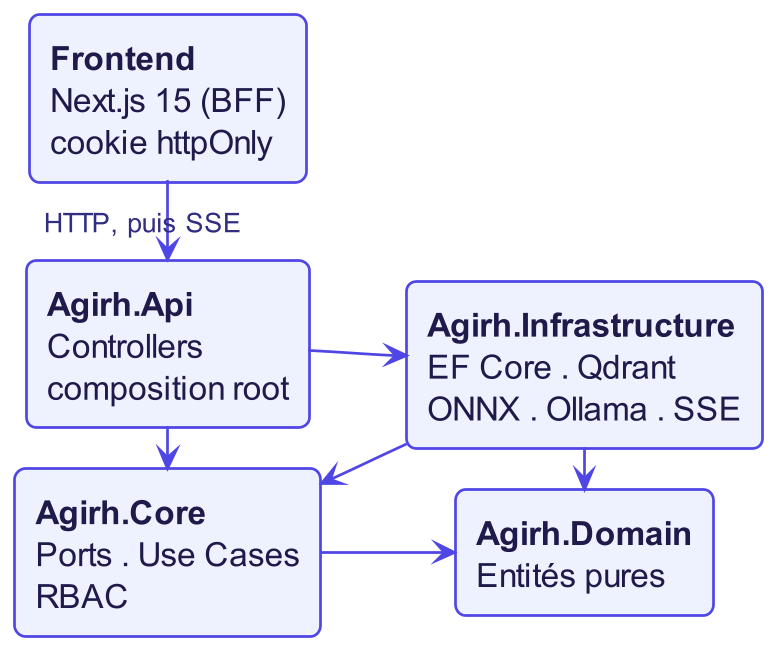
\includegraphics[width=0.58\textwidth]{architecture.png}
\end{center}

\vspace{-4pt}
\begin{center}\small
\begin{tabularx}{\textwidth}{@{}l X@{}}
\toprule
\textbf{Composant} & \textbf{Choix et usage} \\
\midrule
Backend & ASP.NET Core, EF Core --- ports/use cases/RBAC dans \code{Agirh.Core}, adaptateurs dans \code{Agirh.Infrastructure} \\
Frontend & Next.js 15, pattern \textbf{BFF} --- le JWT n'est jamais expos\'e au navigateur, cookie \code{httpOnly} pos\'e c\^ot\'e serveur \\
Auth \& RBAC & JWT + ASP.NET Identity, 3 r\^oles (\code{Employee}/\code{HR}/\code{QualityAdmin}), port\'ee RH v\'erifi\'ee \emph{avant} le r\^ole (\code{DepartmentScopeGuard}) \\
Temps r\'eel & SSE (Server-Sent Events) --- un seul m\'ecanisme pour le chat en streaming et les notifications \\
Donn\'ees & SQL Server (entit\'es m\'etier) + \textbf{Qdrant} (index vectoriel RAG, ANN/HNSW, cosinus) \\
D\'eploiement & Docker Compose (4 services), Ollama natif sur l'h\^ote (accès GPU/mod\`eles entreprise) \\
\bottomrule
\end{tabularx}
\end{center}

% ---------- 3. IA ----------
\newpage
\section{Le c\oe{}ur du projet : le sous-syst\`eme IA}

\subsection{Pipeline RAG --- 4 phases obligatoires}
\begin{enumerate}
  \item \textbf{Chunking structurel} (sections Markdown, pas de d\'ecoupage \`a taille fixe) : budget de 400 tokens/chunk avec 15\% de recouvrement entre chunks voisins, pour ne jamais perdre une information \`a cheval sur une fronti\`ere de d\'ecoupage.
  \item \textbf{Embedding} multilingue (corpus en fran\c{c}ais) en \textbf{ONNX Runtime .NET pur}, 768 dimensions --- aucun appel Ollama pour cette \'etape, contr\^ole total de la latence.
  \item \textbf{Storage} \textbf{Qdrant}, recherche ANN/HNSW en similarit\'e cosinus --- corpus r\'eel index\'e et v\'erifi\'e (6 documents $\rightarrow$ 72 chunks).
  \item \textbf{Reranking} cross-encodeur ONNX (\code{bge-reranker-v2-m3}) --- phase obligatoire, pas une am\'elioration optionnelle : c'est elle qui distingue un vrai pipeline RAG d'un RAG na\"if. Un score \'elev\'e mesure une proximit\'e th\'ematique, jamais une preuve que la r\'eponse est pr\'esente --- le seuil de pertinence (0,01) sert de filtre de bruit, pas de garantie \`a lui seul.
\end{enumerate}

\subsection{Orchestration et garde-fou anti-hallucination}
Un \textbf{Router} (Ollama, \code{phi4-mini:3.8b}) classe chaque question en trois intentions. Sa sortie n'est \textbf{jamais} utilis\'ee telle quelle : valid\'ee contre un enum ferm\'e, tout ce qui ne correspond pas exactement retombe sur \emph{hors p\'erim\`etre} par d\'efaut --- \textbf{fail-safe, pas fail-open}.

Le point le plus important du projet : \textbf{deux portes de sortie anticip\'ee}, \emph{en code}, avant tout appel au \textbf{Generator}. Si Qdrant ne retourne aucun candidat, ou si aucun ne passe le seuil de pertinence apr\`es reranking, le Generator n'est jamais invoqu\'e --- le syst\`eme r\'epond directement qu'il n'a pas trouv\'e l'information. Ce n'est pas une consigne de prompt que le mod\`ele pourrait ignorer : c'est v\'erifiable et couvert par des tests d\'edi\'es.

\begin{center}
  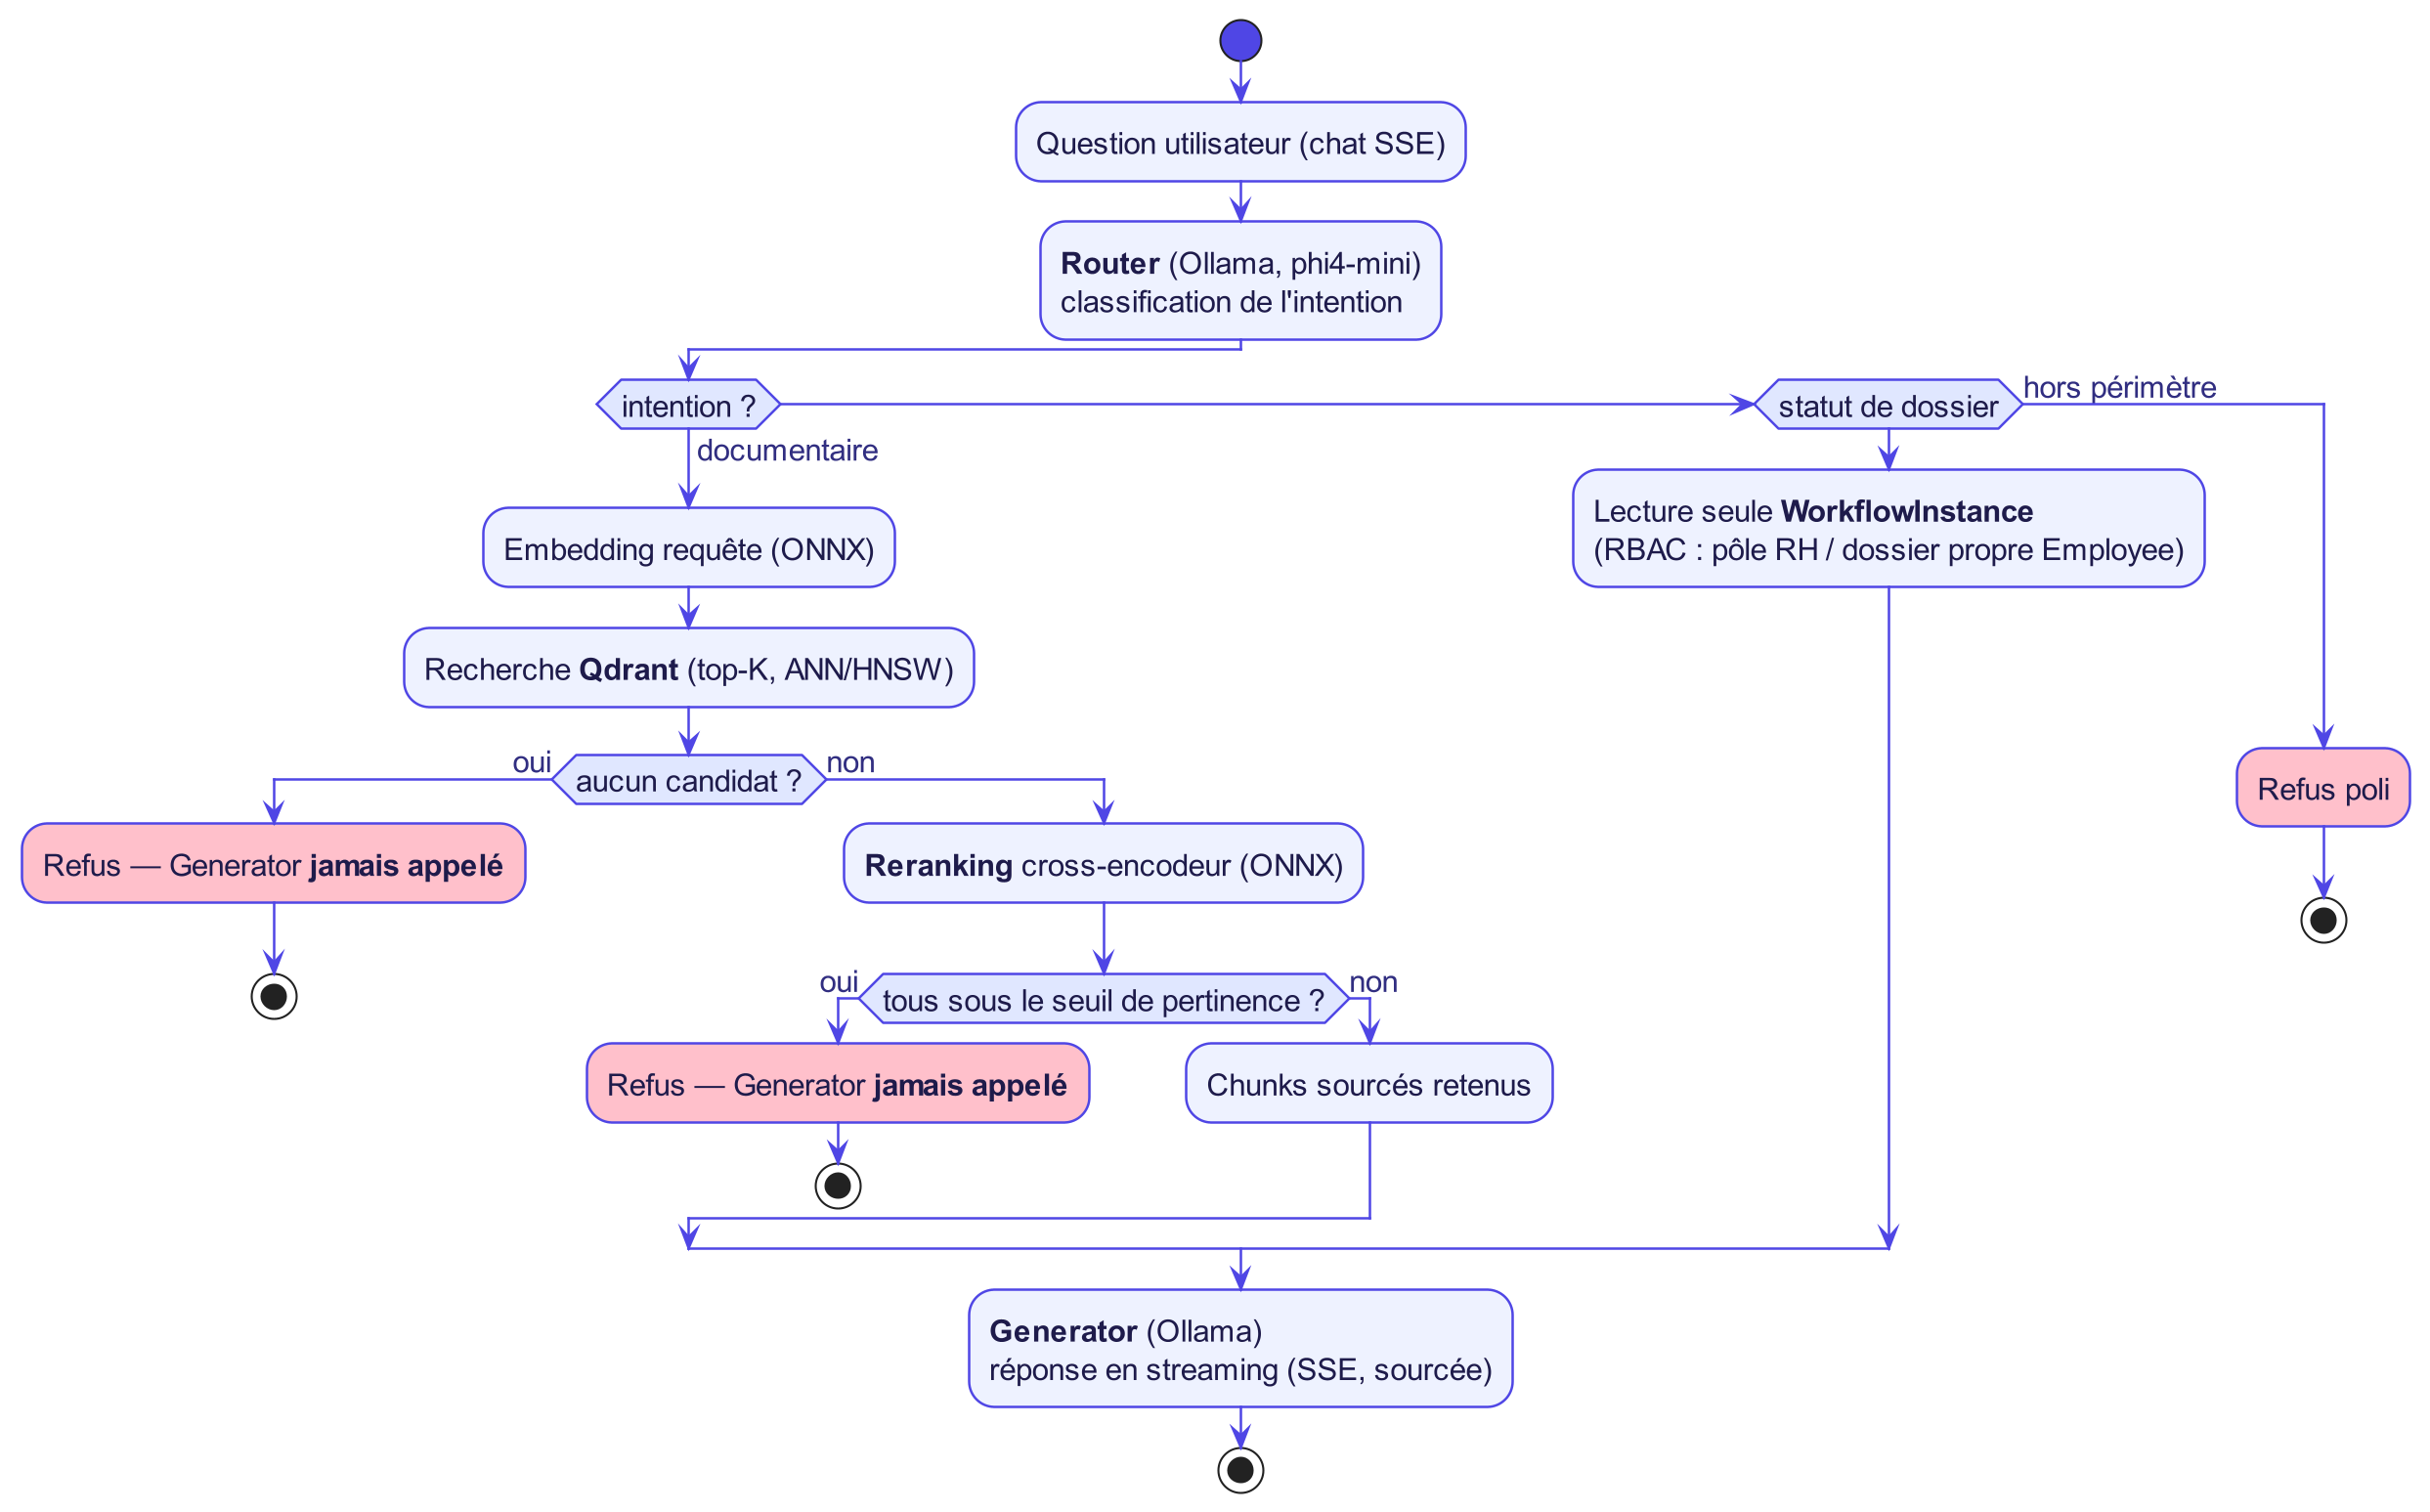
\includegraphics[width=0.72\textwidth]{ai_pipeline.png}
\end{center}

\textit{Limite mesur\'ee et assum\'ee} : le Router se trompe sur $\sim$27\% d'un jeu de 48 questions test (isol\'e derri\`ere un port, sans impact sur le garde-fou anti-hallucination). Doubler les exemples few-shot n'a eu aucun effet mesur\'e --- limite de raisonnement d'un mod\`ele 3,8B, document\'ee plut\^ot que masqu\'ee.

% ---------- 4. Workflows ----------
\newpage
\section{Workflows m\'etier}

\textbf{Onboarding} : le RH du p\^ole cr\'ee une fiche collaborateur (Poste, P\^ole, Contrat, Date) $\rightarrow$ r\'esolution des items attendus contre le \emph{template approuv\'e} correspondant (crois\'e Poste $\times$ P\^ole $\times$ Contrat) $\rightarrow$ \code{WorkflowInstance} + checklist persist\'ees $\rightarrow$ items coch\'es ind\'ependamment (audit trail) $\rightarrow$ cl\^oture puis archivage en lecture seule d\'efinitive.

\textbf{Circuit qualit\'e des templates} : un RH \textbf{propose} $\rightarrow$ un Admin/Qualit\'e \textbf{v\'erifie} $\rightarrow$ un second \textbf{approuve} --- seul un template \emph{Approved} peut instancier un dossier r\'eel, contrainte v\'erifi\'ee par le code, pas seulement document\'ee. Trois r\^oles distincts emp\^echent qu'une seule personne valide unilat\'eralement son propre travail.

\begin{center}
  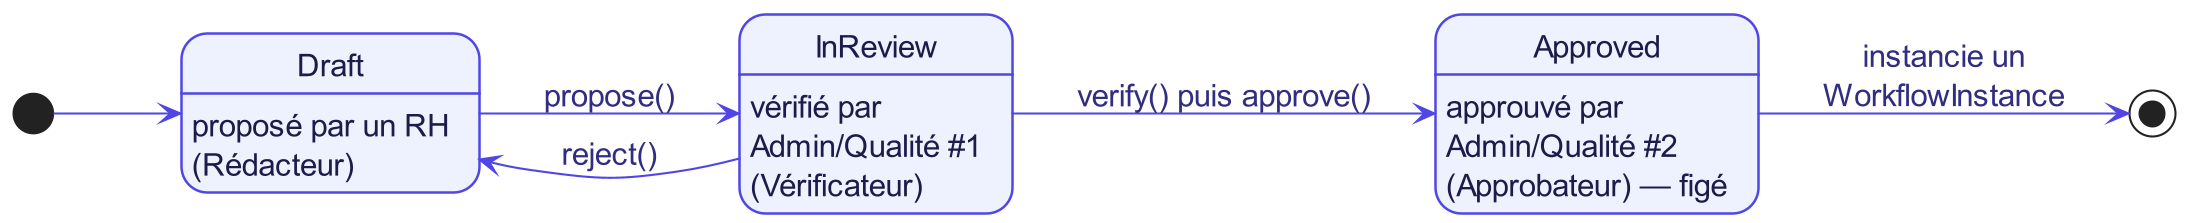
\includegraphics[width=0.92\textwidth]{workflow_circuit.png}
\end{center}

% ---------- 5. Bilan ----------
\section{Bilan v\'erifi\'e et suite}

\textbf{211 tests automatis\'es} (xUnit/Moq/FluentAssertions), \textbf{0 warning} au build. Pipeline RAG et orchestration v\'erifi\'es en HTTP r\'eel de bout en bout (ingestion $\rightarrow$ question $\rightarrow$ r\'eponse sourc\'ee, streaming token par token). D\'eploiement Docker Compose (4 services + Ollama natif) v\'erifi\'e sur base fra\^iche : inscription $\rightarrow$ connexion $\rightarrow$ chat sourc\'e, de bout en bout.

\textit{Suite pr\'evue} : affiner le Router (nouvelle approche \`a \'evaluer, le simple ajout d'exemples n'ayant pas suffi) ; endpoints de lecture/liste pour des vues RH au-del\`a du chat ; trois cas particuliers m\'etier encore ouverts (mutation inter-p\^ole, annulation/suspension, p\^ole vacant).

\end{document}
